\section{Variables aleatorias discretas y su relación con ciencia de datos}
\subsection{Distribuciones discretas y su relación con ciencia de datos}

Las distribuciones discretas estudiadas en este capítulo no son solo objetos teóricos: son herramientas fundamentales en el análisis y modelado de datos. A continuación se resumen sus aplicaciones más comunes en ciencia de datos.

\begin{itemize}
 \item \textbf{Distribución binomial:} Se utiliza en pruebas A/B para determinar si existe una diferencia estadísticamente significativa entre dos tasas de conversión. También es la base de muchos modelos de clasificación binaria.

 \item \textbf{Distribución de Poisson:} Modela la frecuencia de eventos raros en un intervalo fijo, como el número de visitas a una página web por minuto, las llamadas a un centro de atención por hora, o los defectos por unidad de producción. Es ampliamente usada en análisis de tráfico y detección de anomalías.

 \item \textbf{Distribución geométrica:} Modela el número de ensayos hasta el primer éxito. En ciencia de datos se aplica en análisis de supervivencia (tiempo hasta la primera conversión), modelado de churn y en el diseño de estrategias de retención.

 \item \textbf{Distribución binomial negativa:} Es una extensión de Poisson que permite modelar datos de conteo con \emph{sobredispersión} (varianza mayor que la media). Es frecuente en datos reales donde la variabilidad excede la predicha por Poisson, por ejemplo en el número de transacciones por cliente o el número de clics por usuario.

 \item \textbf{Distribución hipergeométrica:} Se emplea cuando se trabaja con muestras sin reemplazo de poblaciones finitas, como en auditorías de calidad, muestreo de encuestas, o en pruebas estadísticas exactas como la prueba exacta de Fisher.
\end{itemize}

\begin{ejemplo}
 \label{exmp:2.10.18}
 Se quiere analizar el número de clicks que reciben $100$ anuncios publicitarios en una hora. Los datos observados tienen media $\bar{x}=4.2$ y varianza $s^{2}=8.7$. ¿Es razonable modelar estos datos con una distribución de Poisson?
\end{ejemplo}

\begin{solucion}
	En una distribución de Poisson, la media y la varianza son iguales: $\mu = \sigma^{2} = \lambda$. Como en este caso $s^{2} = 8.7 \gg \bar{x} = 4.2$, los datos presentan \emph{sobredispersión}. Por lo tanto, una distribución de Poisson \emph{no} es adecuada. En su lugar, se recomienda usar una distribución binomial negativa, que permite modelar esta variabilidad adicional.
\end{solucion}

\lstinputlisting[language=Python]{../code/distribuciones-especiales/distDataScience.py}

\begin{figure}
 \centering
 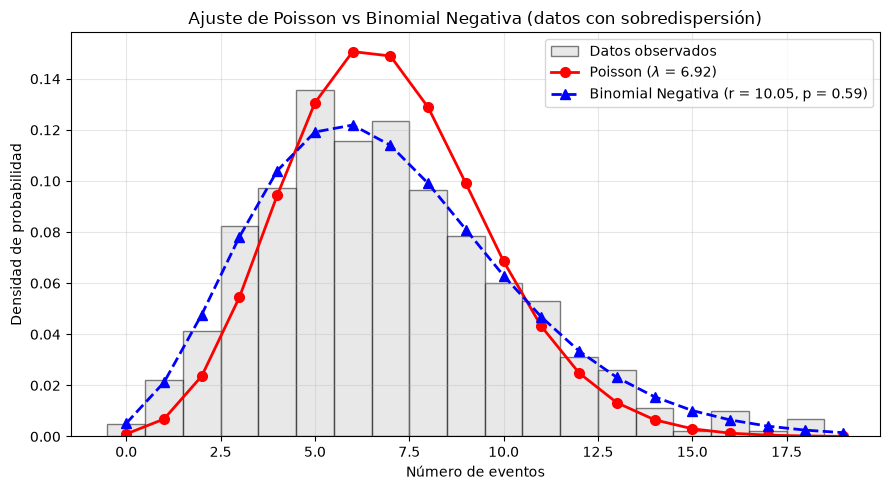
\includegraphics[height=7cm,keepaspectratio=true]{./pe/distDataScience.png}
 % distDataScience.png: 0x0 pixel, 300dpi, 0.00x0.00 cm, bb=
 \caption{Comparación de ajuste de Poisson vs. Binomial Negativa para datos con sobredispersión}
 \label{fig:2.10.10}
\end{figure}

\begin{observacion}
	En la práctica, la elección de la distribución depende tanto de la naturaleza del fenómeno modelado como de las propiedades estadísticas de los datos observados. Herramientas como la función de verosimilitud, el criterio de información de Akaike (AIC) o validación cruzada permiten comparar distintos modelos y elegir el más apropiado.
\end{observacion}

